\documentclass{standalone}
\usepackage{tikz}
\usetikzlibrary{trees,positioning}
\begin{document}
\sffamily
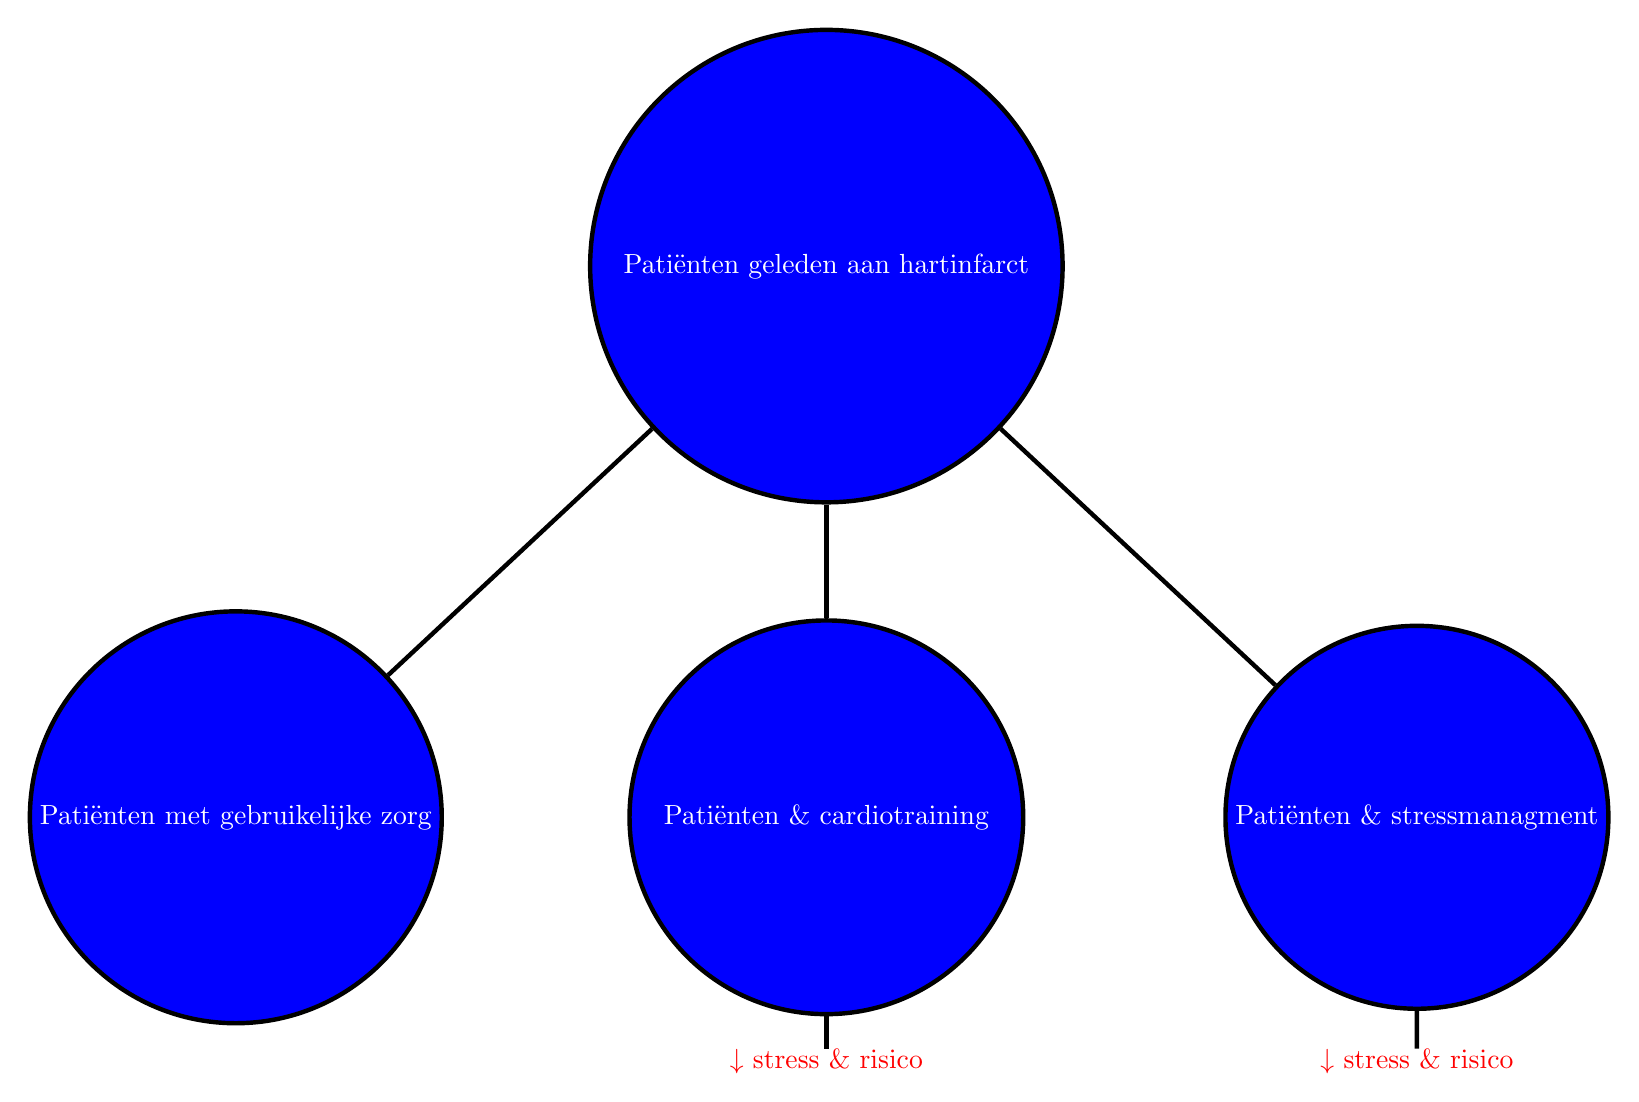
\begin{tikzpicture}[bal/.style={circle,fill=blue,minimum size=6.0cm, text=white,draw, ultra thick,align=center},level 1/.style={level distance=7cm, sibling distance=7.5cm},
	level 2/.style={sibling distance=3cm,level distance=3.1cm},
	level 3/.style={sibling distance=3cm,level distance=3.1cm},
	edge from parent/.style={draw,ultra thick},
]
\node[bal] {Patiënten geleden aan hartinfarct}
    child {node[bal,minimum size=4.0cm] {Patiënten met gebruikelijke zorg}}
    child {node[bal,minimum size=5.0cm] {Patiënten \& cardiotraining}
        child{node[minimum size=0.0cm,inner sep=0,text=red] {$\downarrow$ stress \& risico}} 
    }
    child {node[bal,minimum size=4.0cm] {Patiënten \& stressmanagment}
        child{node[inner sep=0,text=red,minimum size=0,] {$\downarrow$ stress \& risico}} 
    }
    ;

\end{tikzpicture}
\end{document}
